\pdfbookmark{Общая характеристика работы}{characteristic}             % Закладка pdf
\section*{Общая характеристика работы}

\newcommand{\actuality}{\pdfbookmark[1]{Актуальность}{actuality}\underline{\textbf{\actualityTXT}}}
\newcommand{\progress}{\pdfbookmark[1]{Разработанность темы}{progress}\underline{\textbf{\progressTXT}}}
\newcommand{\aim}{\pdfbookmark[1]{Цели}{aim}\underline{{\textbf\aimTXT}}}
\newcommand{\object}{\pdfbookmark[1]{Объектом исследования}{object}\underline{\textbf{\objectTXT}}}
\newcommand{\objective}{\pdfbookmark[1]{Предметом исследования}{objective}\underline{\textbf{\objectiveTXT}}}
\newcommand{\tasks}{\pdfbookmark[1]{Задачи}{tasks}\underline{\textbf{\tasksTXT}}}
\newcommand{\aimtasks}{\pdfbookmark[1]{Цели и задачи}{aimtasks}\aimtasksTXT}
\newcommand{\novelty}{\pdfbookmark[1]{Научная новизна}{novelty}\underline{\textbf{\noveltyTXT}}}
\newcommand{\influence}{\pdfbookmark[1]{Практическая значимость}{influence}\underline{\textbf{\influenceTXT}}}
\newcommand{\methods}{\pdfbookmark[1]{Методология и методы исследования}{methods}\underline{\textbf{\methodsTXT}}}
\newcommand{\defpositions}{\pdfbookmark[1]{Положения, выносимые на защиту}{defpositions}\underline{\textbf{\defpositionsTXT}}}
\newcommand{\reliability}{\pdfbookmark[1]{Достоверность}{reliability}\underline{\textbf{\reliabilityTXT}}}
\newcommand{\probation}{\pdfbookmark[1]{Апробация}{probation}\underline{\textbf{\probationTXT}}}
\newcommand{\contribution}{\pdfbookmark[1]{Личный вклад}{contribution}\underline{\textbf{\contributionTXT}}}
\newcommand{\publications}{\pdfbookmark[1]{Публикации}{publications}\underline{\textbf{\publicationsTXT}}}

{\actuality} 
%Обзор, введение в тему, обозначение места данной работы в
%мировых исследованиях и~т.\:п., можно использовать ссылки на~другие
%работы~\autocite{Gosele1999161,Lermontov}
%(если их~нет, то~в~автореферате
%автоматически пропадёт раздел <<Список литературы>>). Внимание! Ссылки
%на~другие работы в~разделе общей характеристики работы можно
%использовать только при использовании \verb!biblatex! (из-за технических
%ограничений \verb!bibtex8!. Это связано с тем, что одна
%и~та~же~характеристика используются и~в~тексте диссертации, и в
%автореферате. В~последнем, согласно ГОСТ, должен присутствовать список
%работ автора по~теме диссертации, а~\verb!bibtex8! не~умеет выводить в~одном
%файле два списка литературы).
%При использовании \verb!biblatex! возможно использование исключительно
%в~автореферате подстрочных ссылок
%для других работ командой \verb!\autocite!, а~также цитирование
%собственных работ командой \verb!\cite!. Для этого в~файле
%\verb!common/setup.tex! необходимо присвоить положительное значение
%счётчику \verb!\setcounter{usefootcite}{1}!.
%Настроить размер изображения с логотипом можно
%в~соответствующих местах файлов \verb!title.tex!  отдельно для
%диссертации и автореферата. Если вам логотип не~нужен, то просто
%удалите файл с~логотипом.

%\ifsynopsis
%Этот абзац появляется только в~автореферате.
%Для формирования блоков, которые будут обрабатываться только в~автореферате,
%заведена проверка условия \verb!\!\verb!ifsynopsis!.
%Значение условия задаётся в~основном файле документа (\verb!synopsis.tex! для
%автореферата).
%\else
%Этот абзац появляется только в~диссертации.
%Через проверку условия \verb!\!\verb!ifsynopsis!, задаваемого в~основном файле
%документа (\verb!dissertation.tex! для диссертации), можно сделать новую
%команду, обеспечивающую появление цитаты в~диссертации, но~не~в~автореферате.
%\fi

%В папке Documents можно ознакомиться в решением совета из Томского ГУ
%в~файле \verb+Def_positions.pdf+, где обоснованно даются рекомендации
%по~формулировкам защищаемых положений.


Системы идентификации автомобилей и регистрации нарушений правил дорожного движения играют важную роль в управлении безопасностью на дорогах, способствуют повышению неотвратимости наказания и снижению смертности в авариях. Существующие системы основаны на видео- или фото-идентификации номеров автомобилей. Работе этих систем могут препятствовать естественные условия или умышленные действия "--- загрязнение при плохих погодных условиях, специальное заслонение номера с помощью листа бумаги или тряпки. В итоге, по сведениям ГИБДД, производительность систем идентификации автомобилей может падать ниже 50~\%. Для борьбы с этим недостатком можно использовать метод радиочастотной идентификации (RFID). При использовании RFID в номерной знак или под лобовое стекло автомобиля помещается специальная радиометка, которая, находясь вблизи RFID-считывателя, передаёт ему свой идентификатор. Подобные системы широко используются при организации бесконтактной оплаты проезда, для контроля доступа персонала, учёта продукции на складах и в магазинах. Хотя существует множество систем рдиочастотной идентификации, особый интерес представляют пассивные системы УВЧ-диапазона 860--960~МГц, в которых метки не обладают собственными источниками энергии и могут быть идентифицированы считывателями на расстоянии порядка 10--20 метров.

Технология RFID давно используется в различных приложениях, связанных с транспортом, однако в этой области по-прежнему остается много неисследованных вопросов. Производительность RFID-систем существенно зависит как от особенностей окружения, распространения радиосигналов и антенн, так и от параметров протокола связи между считывателем и метками EPC Class 1 Generation 2 (EPC Gen2), основанного на протоколе ALOHA. Хотя анализу производительности систем радиочастотной идентификации в различных приложениях посвящено немало работ, тема применения RFID для идентификации автомобилей остается менее изученной с теоретической точки зрения. Для получения адекватной оценки производительности необходимо создание моделей, учитывающих как параметры распространения радиосигналов, так и всевозможные настройки считывателей и параметры протокола.

Для работы автоматической безопасности необходимо соединять точки идентификации с центрами обработки данных телекоммуникационными сетями, по которым оперативно передается информация о распознанных автомобилях. Проводные решения оказываются не всегда доступными по техническим (отсутствие каналов связи вблизи точек установки, перегруженность имеющихся каналов) или экономическим (дороговизна создания протяженных линий связи) соображениям, поэтому особый интерес представляют беспроводные сети. Такие сети имеют низкую стоимость и быстро строятся, однако их производительность может быть невысокой. Для анализа проивзодительности беспроводных сетей часто применяются стохастические методы, но из-за высокой сложности их зачастую трудно применять для анализа больших многошаговых сетей. Одним из наиболее распространённых методов исследований являются сети массового обслуживания (СеМО), в которых каналы связи и маршрутизаторы моделируются обслуживающими приборами с очередями. В частности, хорошую точность при описании реальных систем показывают СеМО с марковсиким входящими потоками (MAP) и распределением времени обслуживания фазового типа (PH). Хотя системы MAP/PH/1/n хорошо исследованы, их применение для построения открытых сетей массового обслуживания, моделирующих реальные беспроводные сети, изучено в меньшей степени. Из-за высокой сложности моделей особый интерес представляют методы быстрого получения приближенных оценок их характеристик.

Для реализации системы радиочастотной идентификации транспорта нужны системы управления и программное обеспечение для связи считывателей с центрами обработки данных. Эти системы обладают рядом особенностей. Во-первых, считыватели могут исчисляться сотнями или тысячами, а передача данных от них должна идти непрерывно. Во-вторых, нужно объединять данные о прочитанных метках с данными от камер. Наконец, для различных служб и ведомств система должна давать разные уровени доступа. Существует множество различных систем и подходов к построению промежуточного программного обеспечения и систем управления считывателями. Кроме исследовательских работ существует ряд стандартов, а также множество готовых коммерческих решений. Однако, большинство из последних адаптированы для применения в иных сценариях (склады, контроль доступа и пр.) и дорого стоят. Кроме того, задача идентификации транспорта обладает рядом специфических особенностей. Из-за этого разработка систем управления считывателями оказывается актуальной.

Исследованиям в области разработки и исследования широкополосных беспроводных сетей и технологии RFID, методам теории массового обслуживания и вопросам ее применения и прочим темам, затрагиваемым в диссертации, посвящен ряд работ, среди которых следует особо отметить работы отечественных и зарубежных учёных: В.М. Вишневский, А.Н. Дудин, П.В. Никитин, А.Е. Кучерявый, К.Е. Самуйлов, Ю.В. Гайдамака, В.В. Рыков, Р.Н. Минниханов, D. Lucantoni, N. Abramson, L.G. Roberts, M.F. Neuts, G. Horvath, G. Bianchi,  H. Okamura, P. Buchholz, M. Telek, J.C. Strelen, L. Bodrog, D. Aldous, K.V.S. Rao, C. Floerkemeier, C. Wang, E. Vahedi, R. Nelson, T.S. Rappaport, S. Singh, J. Kriege, P. Djukic, S. Valaee, J.E. Hoag. и др.

% {\progress}
% Этот раздел должен быть отдельным структурным элементом по
% ГОСТ, но он, как правило, включается в описание актуальности
% темы. Нужен он отдельным структурынм элемементом или нет ---
% смотрите другие диссертации вашего совета, скорее всего не нужен.

{\object} являются системы радиочастотной идентификации транспорта и опорные многошаговые беспроводные сети. {\objective} являются методы анализа и алгоритмы расчета характеристик производительности систем радиочастотной идентификации и многошаговых беспроводных сетей, а также методы построения систем управления распределенными системами идентификации транспорта.

{\aim} данной работы является создание комплекса моделей для анализа производительности систем радиочастотной идентификации и широкополосных беспроводных сетей, а также разработка и экспериментальное внедрение системы управления и сбора данных с RFID-считывателей.

Для~достижения поставленной цели было необходимо решить следующие {\tasks}:
\begin{enumerate}[beginpenalty=10000] % https://tex.stackexchange.com/a/476052/104425
  \item Разработать комплекс аналитических и имитационных моделей для анализа производительности систем радиочастотной идентификации транспортных средств, позволяющих адекватно оценивать их производительность.
  \item Разработать комплекс аналитических моделей на базе методов теории массового обслуживания для оценки производительности опорных беспроводных сетей с использованием марковских случайных потоков для моделирования трафика и распределений фазового типа для моделирования процесса передачи данных, а также методов понижения размерности для нахождения эффективных способов расчёта показателей производительности.
  \item Разработать распределенную систему управления и сбора данных с RFID-считывателей и провести её экспериментальное внедрение.
\end{enumerate}


{\novelty}
\begin{enumerate}[beginpenalty=10000] % https://tex.stackexchange.com/a/476052/104425
  \item Впервые была предложена стохастическая модель системы радиочастотной идентификации с мобильными метками, учитывающая различные законы движения меток, а также сценарии переключения питания и смены опрашиваемых значений флагов сессий.
  \item Был разработан новый комплекс аналитических и имитационных моделей для анализа вероятности идентификации быстро движущихся транспортных средств с учетом особенностей логического и физического уровней EPC Gen2, а также учитывающих особенности распространения радиосигналов вблизи автодороги.
  \item Были предложены методы построения сетей массового обслуживания с марковскими входными потоками и распределениями фазового типа для моделирования многошаговых беспроводных сетей, учитывающие возникновение коллизий при передаче пакетов, и впервые был исследован метод расчета их характеристик методом понижения размерности входящих потоков. В численном эксперименте показано, в каких случаях эти модели позволяют получить адекватные оценки производительности беспроводной сети.
  \item Была разработана и реализована распределенная система управления RFID-считывателями, предназначенная для организации сбора данных об идентифицированных транспортных средствах и допускающая объединение с данными, поступающими от прочих источников идентификации.
  \item Было проведено два эксперимента по внедрению системы радиочастотной идентификации в городских условиях и получены экспериментальные данные об эффективности такой системы.
\end{enumerate}

{\influence} Аналитические модели протокола EPC Gen2, предложенные в работе, могут использоваться для первоначальной оценки производительности системы радиочастотной идентификации движущихся автомобилей при различных режимах работы считывателя. Имитационная модель этой системы, учитывающая особенности протокола, оборудования и канала связи между считывателем и метками, может использоваться для получения достаточно точных оценок производительности системы при различных интенсивностях и скоростях дорожного движения.

Модели многошаговых беспроводных сетей могут использоваться для оценки производительности (межконцевых задержек и вероятностей потери пакетов) при проектировании сетей, используемых для сбора данных со считывателей или видеокамер, регистрирующих проезды автомобилей.

Распределенная система управления считывателями и промежуточное программное обеспечение, описанные в работе, использовались в двух экспериментах в городе Казань: при проведении широкомасштабного эксперимента по применению радиочастотной идентификации на дорогах общего пользования в 2014 году, а также при испытаниях на полигоне весной 2020 года. Предложенные решения могут использоваться при дальнейшем практическом внедрении системы радиочастотной идентификации автомобилей.

Результаты работы также были использованы в исследованиях, проводимых по следующим грантам:

\begin{itemize}
	\item Контракт c Министерством образования и науки РФ № 14.514.11.4071 в рамках федеральной целевой программы <<Исследования и разработки по приоритетным направлениям развития научно-технологического комплекса России на 2007-2013 годы>> поисковые научно-исследовательские работы по лоту шифр <<2013-1.4-14-514-0122>> <<Разработка технологии и архитектуры аппаратно-программных средств сверхвысокоскоростных беспроводных сетей в миллиметровом диапазоне радиоволн 60-100 ГГц>> по теме: <<Разработка и исследование технологии и архитектуры сверхвысокоскоростных беспроводных сетей в миллиметровом Е-диапазоне радиоволн 71-76 ГГц, 81-86 ГГц>>
	\item Соглашение с Министерством образования и науки РФ о предоставлении субсидии от 22.10.2014 г. № 14.613.21.0020 в рамках федеральной целевой программы <<Исследования и разработки по приоритетным направлениям развития научно-технологического комплекса на 2014-2020 годы>> по теме: <<Разработка математических методов, алгоритмов и программ оценки производительности и проектирования широкополосных беспроводных сетей передачи мультимедийной информации вдоль протяженных транспортных магистралей (железнодорожное полотно, автодороги) и трубопроводов (нефтяные и газовые магистрали)>>
	\item Грант Российского научного фонда (РНФ) № 16-49-02021 <<Новый комплекс математических моделей, методов, алгоритмов и программ управляемых стохастических систем для оценки производительности и проектирования телекоммуникационных сетей следующего поколения>>
	\item Грант Российского фонда фундаментальных исследований (РФФИ) № 13-07-00737 <<Разработка принципов построения и математических методов исследования нового класса автоматизированных систем безопасности на автодорогах с использованием RFID-технологий и высокоскоростной беспроводной связи>> 
	\item Грант Российского фонда фундаментальных исследований (международный проект РФФИ "--- БРФФИ) № 14-07-90015 Бел\_а <<Разработка и исследование методов оценки производительности и проектирования гибридных систем передачи мультимедийной информации на базе лазерной и радио технологий>>
	\item Грант Российского фонда фундаментальных исследований (международный проект РФФИ "--- БРФФИ) № 16-57-00130 Бел\_а <<Разработка и исследование методов синтеза архитектуры широкополосных беспроводных сетей с линейной топологией>>
\end{itemize}

{\methods} Для решения задач, поставленных в диссертации, использовались методы теории вероятности, математической статистики, теории случайных процессов, теории массового обслуживания, методы моделирования беспроводных протоколов и сетей с помощью марковских цепей, методы дискретно-событийного имитационного моделирования. При разработке программного обеспечения использовались методоы многопоточного программирования, методы разработки распределенных систем.

{\defpositions}
\begin{enumerate}[beginpenalty=10000] % https://tex.stackexchange.com/a/476052/104425
  \item Разработка тохастической модели системы радиочастотной идентификации с мобильными метками, учитывающей различные законы движения меток, а также сценарии переключения питания и смены опрашиваемых значений флагов сессий.
  \item Разработка комплекса аналитических и имитационных моделей для анализа вероятности идентификации быстро движущихся транспортных средств с учетом особенностей логического и физического уровней EPC Gen2, а также учитывающего особенности распространения радиосигналов вблизи автодороги.
  \item Разработка комплекса аналитических и имитационных моделей многошаговых беспроводных сетей на основе открытых сетей массового обслуживания с марковскими входными потоками и распределением времени обслуживания фазового типа, позволяющего быстро рассчитывать характеристики сети с помощью метода сокращения пространства состояний.
  \item Разработка распределенной системы управления RFID-считывателями, применимой для создания систем радиочастотной идентификации автотранспорта. Практическое подтверждение эффективности разработанного прототипа в ходе экспериментального внедрения системы радиочастотной идентификации в городе Казань. 
\end{enumerate}

{\reliability} полученных результатов обеспечивается использованием строгих математических моделей, сравнением результатов аналитического и имитационного моделирования. Результаты анализа вероятности идентификации автомобилей согласуются с результатами, полученными в ходе реального крупномасштабного эксперимента. Результаты находятся в соответствии с результатами, полученными другими авторами.


{\probation}
основные результаты работы докладывались~на следующих конференциях: 12th Annual IEEE International conference on RFID 2018 (IEEE RFID 2018; США, Орландо); 11th Annual IEEE International conference on RFID 2017 (IEEE RFID 2017; США, Финикс); международный форум Kazan Digital Week 2020 (Казань); International conference on Advances in Applied Probability and Stochastic Processes 2019 (ICAAP \& SP 2019; Индия, Коттаям); 13-е и 12-е Всероссийские совещания по проблемам управления (ВСПУ 2019, ВСПУ 2014; Москва, ИПУ РАН); 18-я, 16-я и 15-я Международные конференции им. А.Ф. Терпугова Информационные технологии и математическое моделирование (ИТММ 2019, ИТММ 2017, ИТММ 2016; Россия); 11th IEEE International Conference on Application of Information and Communication Technologies (IEEE AICT 2017; Москва, ИПУ РАН); 21-я, 20-я, 19-я, 18-я и 17-я Международные Конференции <<Распределенные компьютерные и телекоммуникационные сети: управление, вычисление, связь>> (DCCN 2018, DCCN 2017, DCCN 2016, DCCN 2015, DCCN 2013; Москва); 7th International Workshop on Communication Technologies for Vehicles (Nets4Cars-Fall 2014; Санкт-Петербург); 2012 International Conference on RFID-Technology and Applications (IEEE RFID-TA 2012; Франция, Ницца); 10-я и 5-я Всероссийская конференция <<Информационно-телекоммуникационные технологии и математическое моделирование высокотехнологичных систем>> (ИТТММ 2020, ИТТММ 2015; Москва, РУДН).

{\contribution} Автор принимал активное участие в разработке стохастической модели протокола EPC Gen2, имитационной модели системы радиочастотной идентификации автомобилей, аналитической и имитационной модели для расчёта производительности многошаговых беспроводных сетей, промежуточного программного обеспечения и системы управления считывателями, разработке считывателя и проведении экспериментов в городе Казань.

\ifnumequal{\value{bibliosel}}{0}
{%%% Встроенная реализация с загрузкой файла через движок bibtex8. (При желании, внутри можно использовать обычные ссылки, наподобие `\cite{vakbib1,vakbib2}`).
    {\publications} Основные результаты по теме диссертации изложены
    в~XX~печатных изданиях,
    X из которых изданы в журналах, рекомендованных ВАК,
    X "--- в тезисах докладов.
}%
{%%% Реализация пакетом biblatex через движок biber
    \begin{refsection}[bl-author, bl-registered]
        % Это refsection=1.
        % Процитированные здесь работы:
        %  * подсчитываются, для автоматического составления фразы "Основные результаты ..."
        %  * попадают в авторскую библиографию, при usefootcite==0 и стиле `\insertbiblioauthor` или `\insertbiblioauthorgrouped`
        %  * нумеруются там в зависимости от порядка команд `\printbibliography` в этом разделе.
        %  * при использовании `\insertbiblioauthorgrouped`, порядок команд `\printbibliography` в нём должен быть тем же (см. biblio/biblatex.tex)
        %
        % Невидимый библиографический список для подсчёта количества публикаций:
        \printbibliography[heading=nobibheading, section=1, env=countauthorvak,          keyword=biblioauthorvak]%
        \printbibliography[heading=nobibheading, section=1, env=countauthorwos,          keyword=biblioauthorwos]%
        \printbibliography[heading=nobibheading, section=1, env=countauthorscopus,       keyword=biblioauthorscopus]%
        \printbibliography[heading=nobibheading, section=1, env=countauthorconf,         keyword=biblioauthorconf]%
        \printbibliography[heading=nobibheading, section=1, env=countauthorother,        keyword=biblioauthorother]%
        \printbibliography[heading=nobibheading, section=1, env=countregistered,         keyword=biblioregistered]%
        \printbibliography[heading=nobibheading, section=1, env=countauthorpatent,       keyword=biblioauthorpatent]%
        \printbibliography[heading=nobibheading, section=1, env=countauthorprogram,      keyword=biblioauthorprogram]%
        \printbibliography[heading=nobibheading, section=1, env=countauthor,             keyword=biblioauthor]%
        \printbibliography[heading=nobibheading, section=1, env=countauthorvakscopuswos, filter=vakscopuswos]%
        \printbibliography[heading=nobibheading, section=1, env=countauthorscopuswos,    filter=scopuswos]%
        %
        \nocite{*}%
        %
        {\publications} Основные результаты по теме диссертации изложены в~\arabic{citeauthor}~печатных изданиях,
        \arabic{citeauthorvak} из которых изданы в журналах, рекомендованных ВАК\sloppy%
        \ifnum \value{citeauthorscopuswos}>0%
            , \arabic{citeauthorscopuswos} "--- в~периодических научных журналах, индексируемых Web of~Science и Scopus\sloppy%
        \fi%
        \ifnum \value{citeauthorconf}>0%
            , \arabic{citeauthorconf} "--- в~тезисах докладов.
        \else%
            .
        \fi%
        \ifnum \value{citeregistered}=1%
            \ifnum \value{citeauthorpatent}=1%
                Зарегистрирован \arabic{citeauthorpatent} патент.
            \fi%
            \ifnum \value{citeauthorprogram}=1%
                Зарегистрирована \arabic{citeauthorprogram} программа для ЭВМ.
            \fi%
        \fi%
        \ifnum \value{citeregistered}>1%
            Зарегистрированы\ %
            \ifnum \value{citeauthorpatent}>0%
            \formbytotal{citeauthorpatent}{патент}{}{а}{}\sloppy%
            \ifnum \value{citeauthorprogram}=0 . \else \ и~\fi%
            \fi%
            \ifnum \value{citeauthorprogram}>0%
            \formbytotal{citeauthorprogram}{программ}{а}{ы}{} для ЭВМ.
            \fi%
        \fi%
        % К публикациям, в которых излагаются основные научные результаты диссертации на соискание учёной
        % степени, в рецензируемых изданиях приравниваются патенты на изобретения, патенты (свидетельства) на
        % полезную модель, патенты на промышленный образец, патенты на селекционные достижения, свидетельства
        % на программу для электронных вычислительных машин, базу данных, топологию интегральных микросхем,
        % зарегистрированные в установленном порядке.(в ред. Постановления Правительства РФ от 21.04.2016 N 335)
    \end{refsection}%
    \begin{refsection}[bl-author, bl-registered]
        % Это refsection=2.
        % Процитированные здесь работы:
        %  * попадают в авторскую библиографию, при usefootcite==0 и стиле `\insertbiblioauthorimportant`.
        %  * ни на что не влияют в противном случае
        \nocite{RFID_JRFID2017}
        \nocite{WINET_IJPAM2016}
        \nocite{WINET_TCOMM2015}
        \nocite{QS_JPU2013}
        \nocite{QS_JITCS2013}
        \nocite{QS_TCOMM2012}

        \nocite{QS_ICAAPSP2020}
        \nocite{QS_ITMM2019}
        \nocite{RFID_IEEERFID2018}
        \nocite{RFID_SYNCHROINFO2018}
        \nocite{RFID_IEEERFID2017}
        \nocite{QS_AICT2017}
        \nocite{QS_ITMM2017}
        \nocite{QS_ITMM2016}
        \nocite{QS_DCCN2016_CCIS}
        \nocite{RFID_DCCN2016_CCIS}
        \nocite{RFIDCTRL_NETS2CARS2014}
        \nocite{RFIDTA2012}
      
        % \nocite{vakbib2}%vak
        % \nocite{patbib1}%patent
        % \nocite{progbib1}%program
        % \nocite{bib1}%other
        % \nocite{confbib1}%conf
    \end{refsection}%
        %
        % Всё, что вне этих двух refsection, это refsection=0,
        %  * для диссертации - это нормальные ссылки, попадающие в обычную библиографию
        %  * для автореферата:
        %     * при usefootcite==0, ссылка корректно сработает только для источника из `external.bib`. Для своих работ --- напечатает "[0]" (и даже Warning не вылезет).
        %     * при usefootcite==1, ссылка сработает нормально. В авторской библиографии будут только процитированные в refsection=0 работы.
}

% При использовании пакета \verb!biblatex! будут подсчитаны все работы, добавленные
% в файл \verb!biblio/author.bib!. Для правильного подсчёта работ в~различных
% системах цитирования требуется использовать поля:
% \begin{itemize}
%         \item \texttt{authorvak} если публикация индексирована ВАК,
%         \item \texttt{authorscopus} если публикация индексирована Scopus,
%         \item \texttt{authorwos} если публикация индексирована Web of Science,
%         \item \texttt{authorconf} для докладов конференций,
%         \item \texttt{authorpatent} для патентов,
%         \item \texttt{authorprogram} для зарегистрированных программ для ЭВМ,
%         \item \texttt{authorother} для других публикаций.
% \end{itemize}
% Для подсчёта используются счётчики:
% \begin{itemize}
%         \item \texttt{citeauthorvak} для работ, индексируемых ВАК,
%         \item \texttt{citeauthorscopus} для работ, индексируемых Scopus,
%         \item \texttt{citeauthorwos} для работ, индексируемых Web of Science,
%         \item \texttt{citeauthorvakscopuswos} для работ, индексируемых одной из трёх баз,
%         \item \texttt{citeauthorscopuswos} для работ, индексируемых Scopus или Web of~Science,
%         \item \texttt{citeauthorconf} для докладов на конференциях,
%         \item \texttt{citeauthorother} для остальных работ,
%         \item \texttt{citeauthorpatent} для патентов,
%         \item \texttt{citeauthorprogram} для зарегистрированных программ для ЭВМ,
%         \item \texttt{citeauthor} для суммарного количества работ.
% \end{itemize}
% % Счётчик \texttt{citeexternal} используется для подсчёта процитированных публикаций;
% % \texttt{citeregistered} "--- для подсчёта суммарного количества патентов и программ для ЭВМ.

% Для добавления в список публикаций автора работ, которые не были процитированы в
% автореферате, требуется их~перечислить с использованием команды \verb!\nocite! в
% \verb!Synopsis/content.tex!. % Характеристика работы по структуре во введении и в автореферате не отличается (ГОСТ Р 7.0.11, пункты 5.3.1 и 9.2.1), потому её загружаем из одного и того же внешнего файла, предварительно задав форму выделения некоторым параметрам

%Диссертационная работа была выполнена при поддержке грантов \dots

%\underline{\textbf{Объем и структура работы.}} Диссертация состоит из~введения,
%четырех глав, заключения и~приложения. Полный объем диссертации
%\textbf{ХХХ}~страниц текста с~\textbf{ХХ}~рисунками и~5~таблицами. Список
%литературы содержит \textbf{ХХX}~наименование.

\pdfbookmark{Содержание работы}{description}                          % Закладка pdf
\section*{Содержание работы}
Во \underline{\textbf{введении}} обосновывается актуальность исследований, проводимых в~рамках данной диссертационной работы, формулируется цель, ставятся задачи работы, излагается научная новизна и практическая значимость представляемой работы, приводится краткое содержание разделов диссертационной работы.

В \underline{\textbf{первой главе}} подробно рассматривается структура распределенной системы радиочастотной идентификации транспорта, описываются основные задачи и проблемы, возникающие при ее построении, анализе производительности и поиске способов увеличения эффективности. Далее приводится обзор современных исследований в областях анализа производительности, способов применения и разработки систем радиочастотной идентификации, методов исследования производительности беспроводных сетей, включая различные сети массового обслуживания. После обзора приводится краткое описание технологии UHF RFID стандарта EPC Class 1 Generation 2 и протоколов беспроводной связи семейства IEEE 802.11, а также радиорелейных линий.

% картинку можно добавить так:
% \begin{figure}[ht]
%     \centerfloat{
%         \hfill
%         \subcaptionbox{\LaTeX}{%
%             \includegraphics[scale=0.27]{latex}}
%         \hfill
%         \subcaptionbox{Knuth}{%
%             \includegraphics[width=0.25\linewidth]{knuth1}}
%         \hfill
%     }
%     \caption{Подпись к картинке.}\label{fig:latex}
% \end{figure}

% Формулы в строку без номера добавляются так:
% \[
%   \lambda_{T_s} = K_x\frac{d{x}}{d{T_s}}, \qquad
%   \lambda_{q_s} = K_x\frac{d{x}}{d{q_s}},
% \]

\underline{\textbf{Вторая глава}} посвящена исследованию производительности системы радиочастотной идентификации движущихся автомобилей. Рассматривается два способа идентификации: по значению EPCID метки, и по паре значений EPCID и TID. Автомобиль считается идентифицированным, если хотя бы одна метка была успешно прочитана хотя бы один раз. В \S~1 приводится описание структуры исследуемой системы радиочастотной идентификации.

В \S~2 приводится первое приближение для расчета вероятности успешной идентификации движущейся со скоростью $v$ метки:
\[
P_t = 1 - \left( 1 - (1 - 2^{-Q})^{N_t-1} (1 - p_e)^L \right)^{N_r},
\]
где $2^Q$ "--- число слотов в раунде опроса, $N_t$ "--- среднее число меток, принимающих участие в раунде, $p_e$ "--- средняя вероятность битовой ошибки (BER), $L$ "--- общее число бит в ответах метки, которые нужно передать для успешной идентификации, $N_r = D / (v T_r)$ "--- среднее число раундов, в которых успевает принять метка, $D$ "--- средняя длина отрезка дороги, на котором метка получает достаточно энергии от считывателя для работы, $v$ "--- скорость движения метки, а $T_r$ "--- средняя длительность раунда инвентаризации. Чем выше длительность символов в командах считывателя и ответах метки, тем ниже BER $p_e$ и выше средняя длительность раундв $T_r$. Реальное значение BER $p_e(t)$, как и величина $D$, меняются со временем, так как из-за эффекта Доплера канал оказывается зависимым от времени.

В \S~3 исследуется зависимость максимальной длительности раундов и числа раундов, в которых принимает участие метки, от параметров протокола EPC Gen.2 (Tari, M, Q и другие). При этом учитывается, что команды считывателя кодируются методом PIE (Pulse-Interval Encoding), в при котором символы нуля и единицы имеют разную длительность.

В \S~4 исследуются затухания прямого и отраженного меткой радиосигналов с использованием двухлучевой модели распространения. При этом учитываются поляризация, диаграммы и коэффициенты усиления антенн, потери при отражении от дороги, потери из-за различных поляризаций, потери на модуляции отраженного сигнала. При вычислении вероятности битовой ошибки (BER) учитывается реальная длительность символов в ответах метки и  возможность ошибки в синхронизации при передаче пруамбулы. Для получения более реалистичной оценки BER используется распределение Рэлея. Из-за того, что считыватель передает сигнал постоянно, кроме краткосрочных периодов отключения, и эффекта Доплера, мощности сигналов и величина BER оказываются сильно зависимыми от времени, прошедшего со включения считывателя. В \S~4 приводятся результаты аналитического расчета величин затухания, BER и мощностей принятых сигналов, а также описываются области, в которых метка получает достаточно энергии для работы. 

\begin{figure}[ht]
  \centerfloat{
    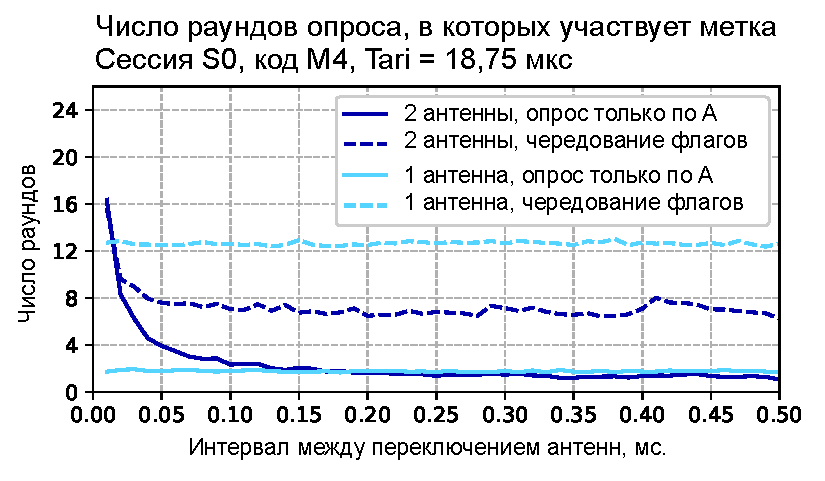
\includegraphics[scale=0.4]{chapter2/ch2_rounds_per_tag.pdf}
  }
  \caption{Число раундов, в которых принимает участие метка}\label{fig:rounds_per_tag}
\end{figure}

В \S~5 приводится краткое описание разработанной имитационной модели, с помощью которой были получены численные оценки вероятности идентификации отдельных меток и автомобилей, а также исследовано число раундов $N_r$, в которых успевает принять метка (см. рис.~\ref{fig:rounds_per_tag}). В имитационной модели учитываются форматы всех команд и ответов, с высокой точностью рассчитываются длительности кадров, мощности сигналов, моделируются отключения питания, переключения антенн и смены сессий опроса меток. Имитационная модель построена на базе экспериментальной системы дискретно-событийного моделирования, разработанной автором на языке Python 3. Для моделирования распространения сигнала используются методы, описанные в разделе \S~4.

\begin{figure}[ht]
  \centerfloat{
    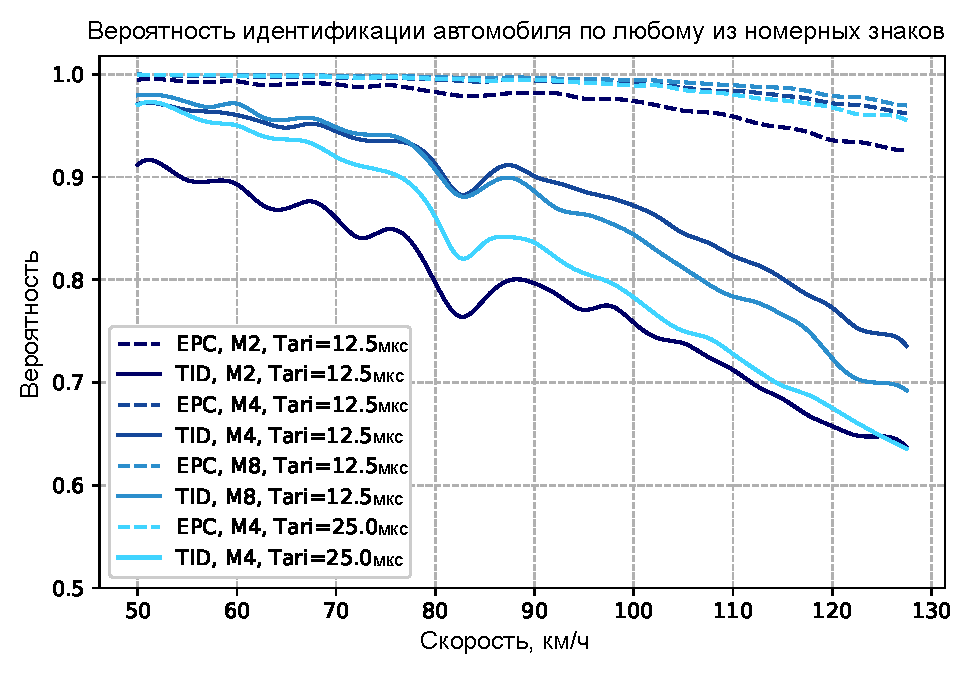
\includegraphics[scale=0.4]{chapter2/ch2_vehicle_identification_rate.pdf}
  }
  \caption{Вероятность успешной идентификации автомобиля}\label{fig:vehicle_identification_rate}
\end{figure}

В разделе \S~6 приведены результаты расчета вероятности идентификации отдельных меток в передних и задних номерах при различных скоростях движения автомобилей и настройках считывателя. Приводится сравнение результатов, полученных с учетом эффекта Доплера и без него, из которых следует, что этот эффект оказывает существенное влияние на эффективность системы, особенно при высоких скоростях движения меток. Также получены результаты расчета вероятности успешной идентификации автомобиля по любой из меток, см. рис.~\ref{fig:vehicle_identification_rate}. Численные эксперименты показывают, что система обладает достаточно высокой эффективностью даже для быстро движущихся автомобилей, когда используются не самые надежные, но и не самые быстрые настройки протокола. При идентификации по EPCID наилучший результат дает использование кода Миллера восьмого порядка (M=8) и Tari = 12,5~мкс, а при идентификации по паре EPCID и TID "--- код Миллера четвертого порядка (M=4) и такое же значение Tari.




\underline{\textbf{Третья глава}} посвящена аналитическому моделированию протокола UHF RFID EPC Class 1 Gen. 2, а именно "--- оценке вероятности идентификации мобильной метки при периодических сменах флагов опроса и сбросах питания считывателем. В \S~1 определяются модельные считыватель и метка, вводятся все основные допущения, использованные в модели, в частности "--- о постоянстве битовой ошибки BER и размере области идентификации, в которой метки включаются, а также о том, что считыватель не передает повторно команды ACK, Req\_Rn или Read при ошибках в ответах меток. В \S~2 главы 3 определяются закон движения меток $x(t)$, функция изменения числа меток в области чтения $f_N(t) = | \{ i: a_i \leqslant t \leqslant a_i + T_L \} |$, где $a_i$ "--- момент входа $i$-й метки в область чтения, $T_L$ "--- время нахождения метки в области чтения, вводятся понятия спецификации раунда и сценария работы считывателя, и приводится формальная постановка задачи. Законы движения меток определяются таким образом, чтобы существовало $\overline{N}$ "--- максимальное число меток в области чтения.

\begin{defn}
\textit{Спецификацией раунда} будем называть пару значений опрашиваемого флага и признака сброса питания $(X, e)$, которую будем сокращенно обозначать символом $\alpha \defeq X^{e}$. \textit{Сценарием работы считывателя} $\bm{\alpha} = \alpha_1 \alpha_2 \dots \alpha_R$ будем называть последовательность спецификаций раундов конечной длины $R$.
\end{defn}

Сценарий работы считывателя определяет периодичность сбросов питания и смены флагов опроса. Считается, что считыватель повторяет свой сценарий в бесконечном цикле.

\begin{probl}\label{probl:analytic_problem}
  Пусть известны законы движения меток $x_i(t) \equiv x(t - t_i)$, вероятность битовой ошибки в передаче ответов $\beta$ и сценарий работы считывателя $\bm{\alpha} = \alpha_1 \alpha_2 \dots \alpha_R$, а также размеры и длительности команд считывателя и ответов меток. Пусть также для идентификации меток требуется только EPCID (или комбинация EPCID и TID). Требуется найти вероятность, с которой каждая метка будет успешно идентифицирована. 
\end{probl}

Для решения задачи \ref{probl:analytic_problem} предлагается описать все изменения, происходящие в системе, в виде композиции пяти элементарных операций: проведения считывателем опроса меток, смены флага опроса меток, сброса питания, добавления и удаления метки из области чтения. Рассматриваются два неоднородных марковских случайных процесса: $\{ \eta_r \}$, моделирующий число \textit{активных} меток в системе (то есть меток, участвующих в раундах), и двумерный процесс $\{ \gamma_r \}$, описывающий число активных меток и состояние выделенной метки. Первый процесс позволяет найти оценку длительностей раундов, второй "--- вычислить вероятность успешной передачи идентификатора выделенной меткой. Оба процесса "--- дискретные, их состояния меняются между раундами опроса. Матрицы переходных вероятностей $D_1, D_2, \dots, D_R$ процесса $\{ \eta_r \}$ и $C_1, C_2, \dots, C_R$ процесс $\{ \gamma_r \}$ определяются числом меток, участвующих в текущем и следующем раундах, и спецификациями этих раундов. 

В \S~3 главы 3 приводится формулы для оценки вероятности, что ровно $m$ из $n$ участвующих в раунде меток ответят на команду ACK $P_n(m) = \sum_{i=m}^n \overline{P}_n(i) {i \choose m}\left( 1 - p_e \right)^m \left( 1 - p_e \right)^{i - m},\; m \leqslant n$, где $\overline{P}_n(i) = \frac{N_s! n!}{i! N_s^n} \sum\limits_{z=0}^{n-i} \frac{(-1)^z (N_s - i - z)^{(n - i - z)}}{(n - i - z)! z! (N_s - i - z)!}$ "--- вероятность того, что ровно $i$ меток из $n$ выберут свободные слоты. 

\begin{equation}\label{eq:round_duration_of_n}
	\tau_r(n) = N_s \sum\limits_{i=0}^{2}p_i(n)t_i + e_r T_\downarrow,
\end{equation}
где $p_i(n), t_i$ "--- вероятности и длительности слотов без ответа ($i = 0$), слотов с успешной передачей идентификатора ($i = 1$) и слотов с ошибками или коллизиями $(i = 2)$, $e_r = 1$, если после раунда считыватель отключает питание на время $T_{\downarrow}$. Средняя длительность раунда при известном распределении числа участвующих меток $\bm{\pi}$ определяется как математическое ожидание 
\begin{equation}\label{eq:avg_round_duration}
  \tau_r = \sum_{i = 0}^{\overline{N}} \pi_i \tau_r(i).
\end{equation}
Также приводится формула для расчета максимальной длительности раунда $\tau_{max}$.

\S~4 главы 3 посвящен проблеме нахождения оценок длительностей раундов $\tau_1, \tau_2, \dots, \tau_R$. Для этого по начальной оценке(полученной, например, исходя из максимальной длительности раундов $\tau_{max}$) и сценарию работы считывателя $\bm{\alpha}$ строится \textit{размеченный сценарий} $\widetilde{\bm{\alpha}} = \widetilde{\alpha}_1 \widetilde{\alpha}_2 \dots \widetilde{\alpha}_R$, символы которого имеют вид $\widetilde{\alpha}_r = X_{N_r}^{e_r}$, где $N_r = f(\tau_1 + \tau_2 + \dots + \tau_{r-1})$ "--- число меток в начале $r$-го раунда. Зная последовательные спецификации $\widetilde{\alpha}_{r}$ и $\widetilde{\alpha}_{r+1}$, можно описать матрицу $D_r$ вероятностей переходов процесса $\eta_r$ в виде произведения матриц элементарных операций $U_N^\nabla$ (проведение опроса с $N$ активными метками), $U_N^\times$ (смена флага опроса), $U_N^\downarrow$ (отключение питания), $U_N^+$ (добавление метки), $U_N^-$ (удаление метки). В произведении $D_r = U_1 U_2 \dots U_l$ самый левый множитель имеет вид $U_{N_r}^\nabla$, остальные "--- в зависимости от значений $N_r$, $N_{r+1}$ и $e_r$. Конкретный вид матриц $U_N$ и способов построения матриц $D_r$, а также примеры описаны в \S~4 главы 3.

Так как считыватель повторяет сценарий своей работы в цикле, делается допущение о том, что аналогично повторяется и размеченный сценарий, то есть после раунда со спецификацией $\widetilde{\alpha}_{R}$ начинается раунд $\widetilde{\alpha}_1$. Тогда для распределения вероятностей $\bm{p}^{(r)}$ процесса $\{ \eta_r \}$ перед $(r + R)$-м раундом выполняется соотношение $\bm{p}^{(r+R)} = \bm{p}^{(r)} D_r D_{r+1} \dots D_R D_1 \dots D_{r-1}$. Подпроцесс $\{ \eta_i^{[r]} \}_{i=0}^\infty$, $\eta_i^{[r]} = \eta_{r+Ri}$, является однородным марковским с матрицей переходных вероятностей $\widetilde{D}_r = D_r D_{r+1} \dots D_R D_1 \dots D_{r-1}$. Для всевозможных подпроцессов $\{ \eta_i^{[r]} \}$, $r = 1, 2, \dots, R$ стационарные вероятности $\bm{\pi}^{(r)}$ вычисляются из следующей системы линейных уравнений:
\begin{equation}\label{eq:bg_pmf_system}
	\begin{cases}
		\bm{\pi}^{(1)} &= \bm{\pi}^{(1)} \widetilde{D}_1\\
		\bm{\pi}^{(2)} &= \bm{\pi}^{(1)} D_1\\
		\dots&\\
		\bm{\pi}^{(R)} &= \bm{\pi}^{(R-1)} D_{R-1}\\
		1              &= \sum\limits_{n=0}^{\overline{N}} \pi^{(1)}_n
	\end{cases}
\end{equation}

С помощью найденных в \eqref{eq:bg_pmf_system} распределений числа активных меток $\bm{\pi}^{(r)}$ и формул для вычисления оценок длительностей раундов \eqref{eq:round_duration_of_n}, \eqref{eq:avg_round_duration} вычисляются новые оценки длительностей раундов $\tau_1, \tau_2, \dots, \tau_R$. Процесс повторяется итерационно до тех пор, пока либо оценки длительностей раундов не перестают меняться более, чем на $\epsilon$, либо не истечет максимальное число итераций алгоритма.

Если исходный сценарий слишком короткий, то при построении расмеченного сценария $\widetilde{\bm{\alpha}}$ используется не сам сценарий $\bm{\alpha}$, а его кратное повторение вида $\bm{\alpha} \bm{\alpha} \dots\, \bm{\alpha}$. Это позволяет учесть изменения числа меток в области чтения, происходящие медленнее, чем смена раундов.

В \S~5 главы 3 описывается построение и анализ двумерного неоднородного марковского случайного процесса $\{ (\eta_r^{[r_0]}, \phi_r^{[r_0]}) \}$, моделирующего прохождение области чтения выделенной меткой, поступившей в область чтения в раунде $r_0$. Компонента $\phi_r^{[r_0]}$ определяет состояние выделенной метки: $\phi_r^{[r_0]} = 0$, если она неактивна, $\phi_r^{[r_0]} = 1$, если метка активна и $\phi_r^{[r_0]} = 2$, если метка хотя бы один раз успешно передала свой идентификатор, это состояние является поглощающим. Процесс является конечным и содержит $Q_{r_0}$ переходов, где $Q_{r_0}$ "--- число раундов, в течение которых наблюдаемая метка находится в области действия считывателя. Тогда вероятность успешной идентификации выделенной метки можно выразить как
\begin{equation}\label{eq:id_prob_phi}
  P_X = \sum\limits_{r \in \mathfrak{R}} p^{[a]}_r \mathbb{P}\{ \phi^{[r]}_{Q_r} = 2 \},
\end{equation}
где $p^{[a]}_{r_0} = \frac{\tau_{r_0}}{\sum_{r \in \mathfrak{R}} \tau_r}$ "--- вероятность поступления выделенной метки в $r_0$-м раунде, а $\mathfrak{R} = \{ r\:|\:r \in [1, R],\; N_{r-1} < N_r \}$ "--- множество таких номеров раундов, в которых происходило увеличение числа меток.

Для удобства, определяется одномерный случайный процесс $\{ \gamma_r^{[r_0]} \}$, состояния которого взаимно однозначно соответствуют состояниям двумерного процесса $\{ (\eta_r^{[r_0]}, \phi_r^{[r_0]}) \}$. Определение матриц переходных вероятностей $C_r^{[r_0]}$, $r = 1, 2, \dots, Q_{r_0}$ процесса $\{ \gamma_r^{[r_0]} \}$ производится аналогично тому, как это было сделано для процесса $\{ \eta_r \}$, однако учитывается дополнительная информация о состоянии одной из меток. Эти матрицы также представляются в виде композиции матриц $V^\nabla_N$, $V^\times_N$, $V^\downarrow_N$, $V^+_N$, $V^-_N$, соответствующих элементарным операциям. Используя найденные матрицы $C_r^{[r_0]}$ можно вычислить вероятность $P_X$ как:

$$
	P_X = \sum\limits_{r_0 \in \mathfrak{R}} p_{r_0}^{[a]} \{ \bm{\theta}^{(r_0,1)} C_1^{[r_0]} C_2^{[r_0]} \dots C_{Q_{r_0}}^{[r_0]} \}_{2\overline{N}+1},
$$
Начальные распределения $\bm{\theta}^{(r_0,1)}$ вычисляются из найденных ранее распределений $\bm{\pi}^{(r)}$:
$$
  \theta_n^{(r_0,1)} = \begin{cases}
    \pi^{(r_0)}_n,                      &\widetilde{\alpha}_{r_0} = A^e_N,\; 1 \leqslant n \leqslant N\\
    \pi^{(r_0)}_{n - (\overline{N}+1)}, &\widetilde{\alpha}_{r_0} = B^e_N,\; \overline{N}+1 \leqslant n \leqslant \overline{N}+N\\
    0,                                  &\text{в остальных случаях.}
  \end{cases}
$$

\begin{figure}[ht!]
  \centerfloat{
    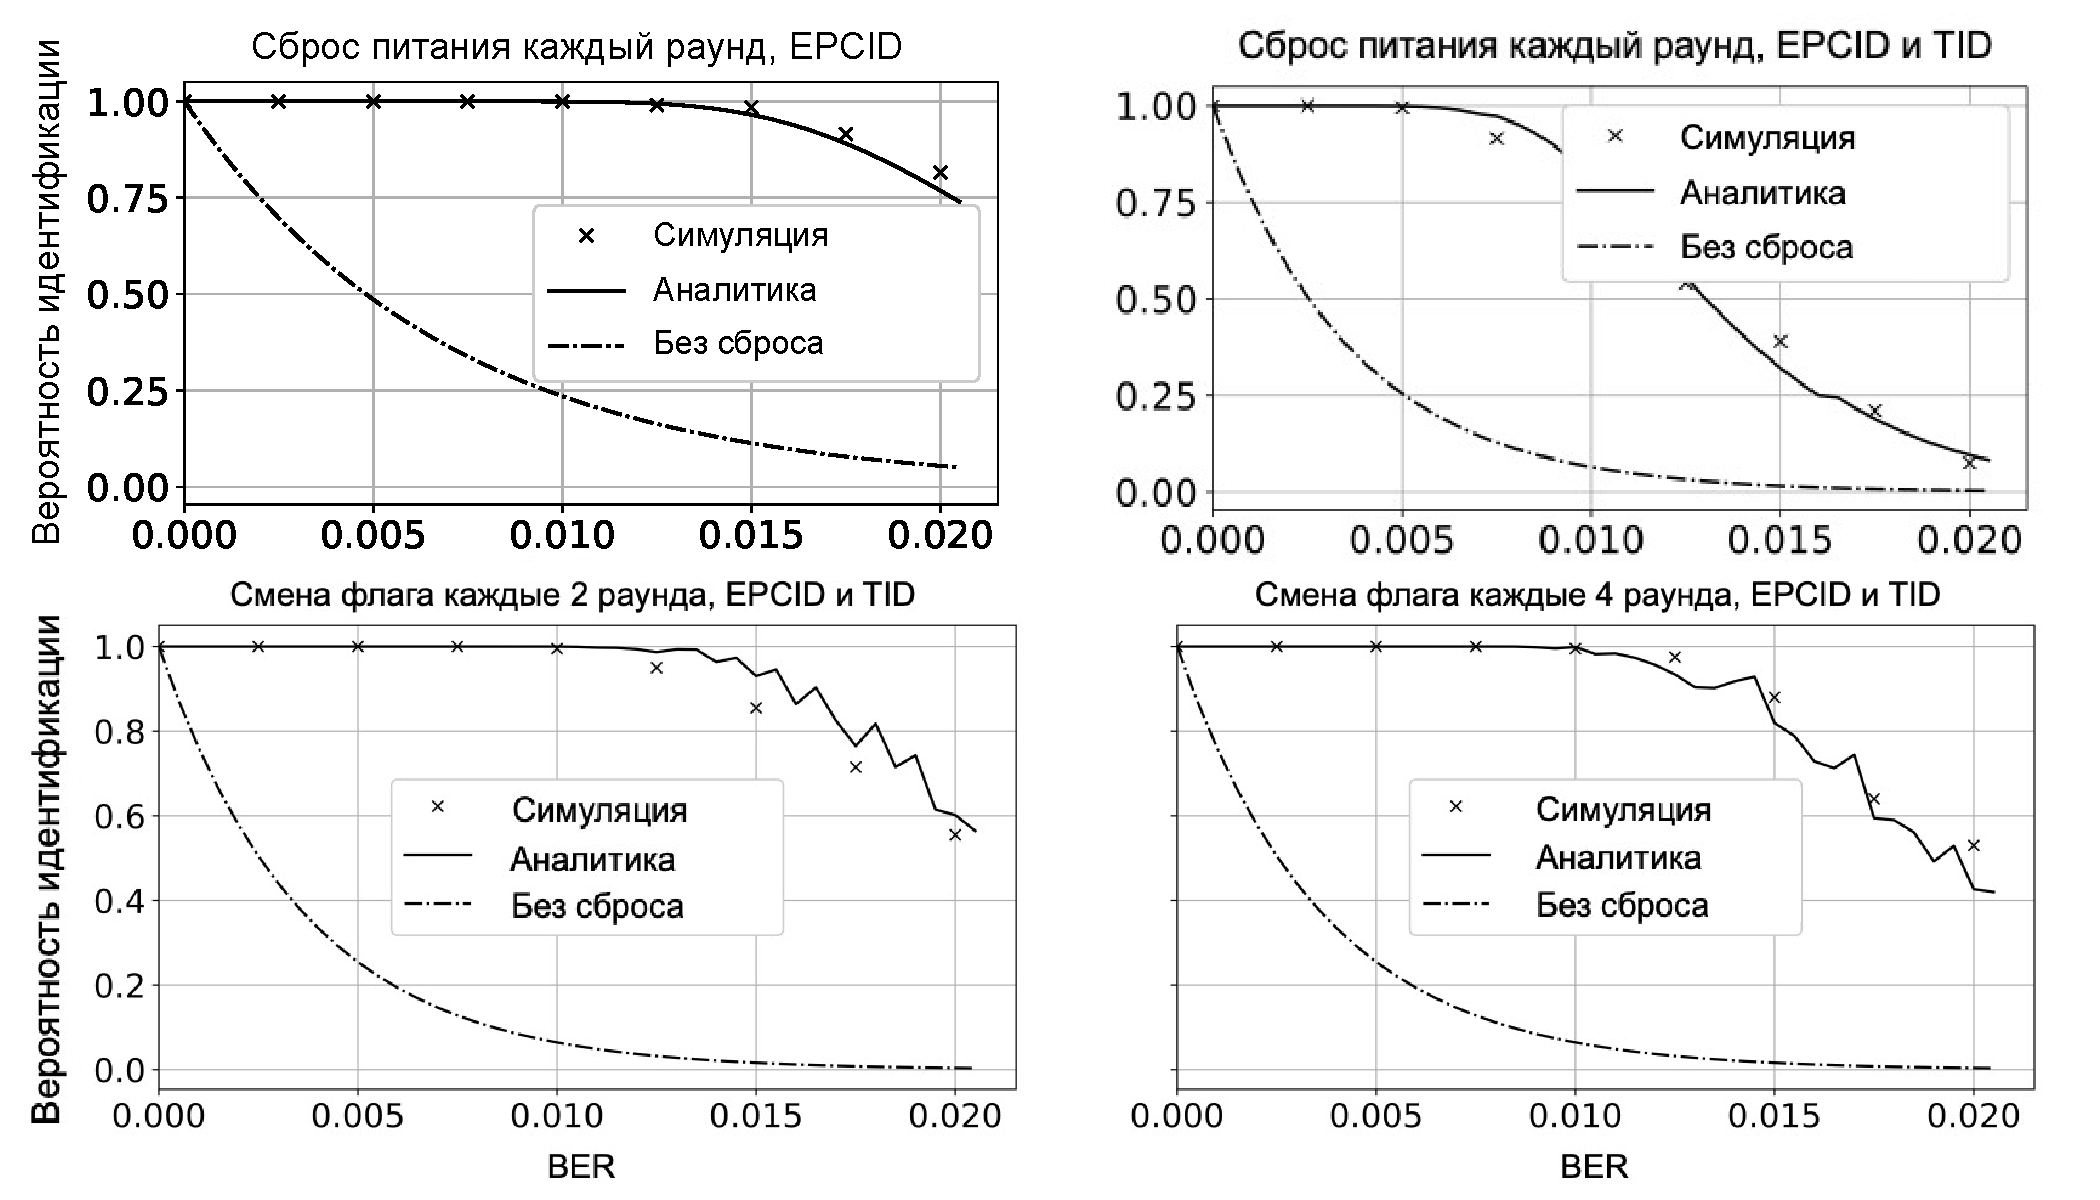
\includegraphics[scale=0.35]{chapter3/ch3_plot_merged.pdf}
  }
  \caption{Вероятность успешной идентификации в разных сценариях работы считывателя}\label{fig:id_prob_var_scenario}
\end{figure}

Численные результаты, полученные с помощью аналитической модели, представлены в \S~6 главы 3. Показано, что периодические сбросы питания и смены флагов опроса ведут к значительному увеличению вероятности успешной идентификации даже при высоких значениях BER, см. рис.~\ref{fig:id_prob_var_scenario}. Результаты аналитического моделирования сравнивались с простой имитационной моделью.


% Можно сослаться на свои работы в автореферате. Для этого в файле
% \verb!Synopsis/setup.tex! необходимо присвоить положительное значение
% счётчику \verb!\setcounter{usefootcite}{1}!. В таком случае ссылки на
% работы других авторов будут подстрочными.
% Изложенные в третьей главе результаты опубликованы в~\cite{vakbib1, vakbib2}.
% Использование подстрочных ссылок внутри таблиц может вызывать проблемы.

\underline{\textbf{Четвертая глава}} посвящена исследованию производительности многошаговых опорных беспроводных сетей с помощью сетей массового обслуживания с узлами типа MAP/PH/1/N. В \S~1 рассматривается классический подход с использованием сетей массового обслуживания с простейшими пуассоновскими потоками и экспоненциальным временем обслуживания и на численном эксперименте демонстрируется, что этот подход дает слишком большую погрешность для многошаговых сетей. Приводится определение системы массового обслуживания с входящими MAP-потоками и PH-распределениями времени обслуживания, излагаются известные результаты о таких системах. Далее приводится описание итерационного алгоритма для расчета характеристик открытой сети массового обслуживания с узалми MAP/PH/1/N и определяется сложность этого алгоритма.

% \begin{figure}[ht!]
%   \centerfloat{
%     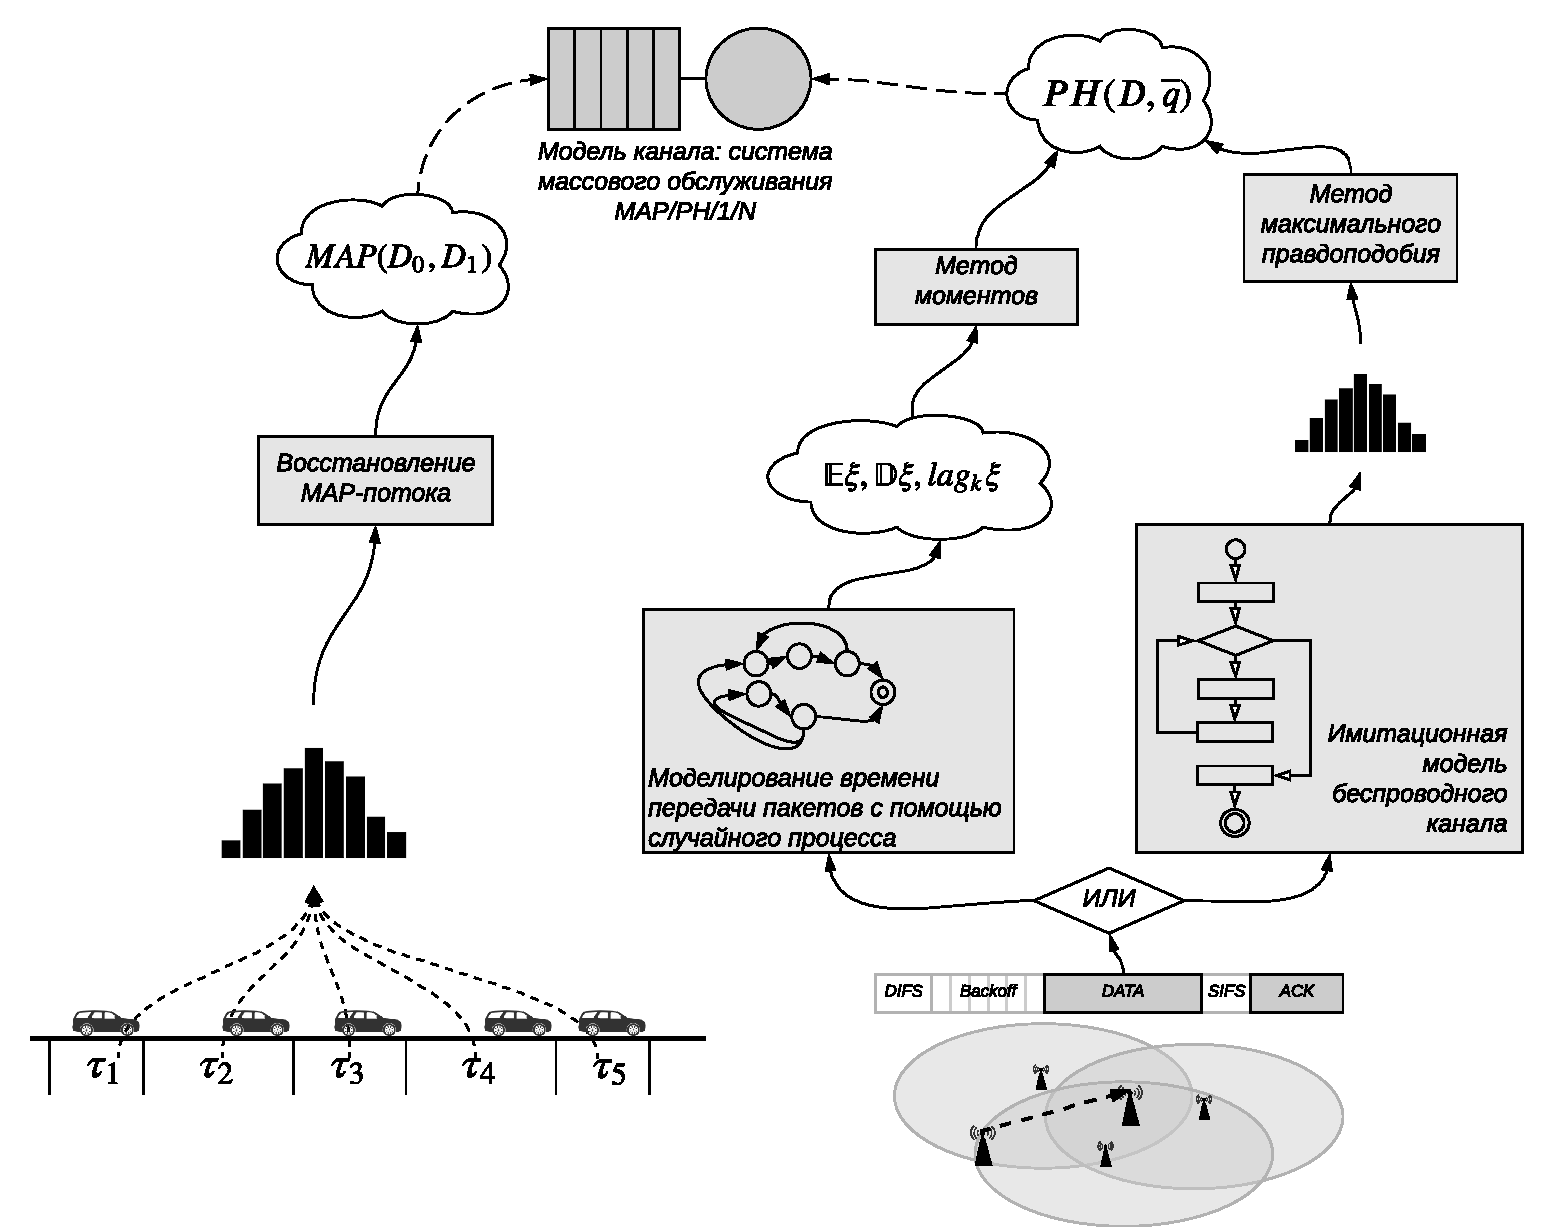
\includegraphics[scale=0.4]{chapter4/ch4_research_schema.pdf}
%   }
%   \caption{Схема моделирования беспроводной сети с помощью сети массового обслуживания с узлами MAP/PH/1/N}\label{fig:qs_schema}
% \end{figure}

\begin{prop}
  Пусть входящие MAP-потоки имеют порядок $W$, PH-распределения "--- порядок $V$, ёмкость очередей равна $M$, и сеть содержит $N$ станций. Тогда итерационная схема расчета характеристик тандемной сети имеет сложность:
  \begin{itemize}
    \item $O((M V W)^{3N})$, если в сети есть кросс-трафик
    \item $O(W^3 (M V)^{3N})$, если кросс-тррафика в сети нет.
  \end{itemize}
\end{prop}

Для эффективного численного расчета характеристик открытой сети массового обслуживания в \S~2 главы 4 приводятся два подхода: метод Монте-Карло, лежащий в основе дискретно-событийной модели сети, и итерационный алгоритм с понижением размерности выходящих MAP-потоков. Понижение размерности производится двумя путями: либо вычислением моментов и коэффициентов автокорреляции выходящего потока и поиска MAP-потока меньшей размерности с этими же характеристиками, либо формированием выборки из приближаемого MAP-потока и применением метода максимизации ожидания (EM-процедуры). В заврешение раздела дается краткая справка об этих методах.

В \S~3 главы 4 описываются подходы к поиску PH-распределений, моделирующих задержки при передаче данных по беспроводному каналу. Рассматриваются схемы передачи данных без конкуренции (для радиорелейных линий) и метод CSMA/CA для беспроводных сетей стандарта IEEE 802.11. Для радиорелейных линий время передачи описывается как сумма случайной величины и нескольких констант. Для каналов IEEE 802.11 рассматривается два варианта работы: в насыщенном режиме, когда у каждой станции есть пакет для передачи, и ненасыщенный режим, когда пакеты поступают в соответствии со случайным распределением. Для моделирования времени передачи в насыщенном режиме предлагается использовать полумарковский случайный процесс, построенный на основе известной модели Bianchi. Для ненасыщенного режима предлагается получать выборки времени с помощью имитационной модели. По вычисленным моментам или выборке величин задержек можно построить PH-распределение, используя либо метод моментов, либо EM-процедуру. Для того, чтобы учесть коллизии в каналах со схемой доступа CSMA/CA, предлагается использовать различные PH-распределения в зависимости от числа конкурирующих станций. В случае опорной сети с линейной топологией, приходится рассматривать три PH-распределения, полученных для станций без соседей, с одним или двумя соседями.

\begin{figure}[ht!]
  \centerfloat{
    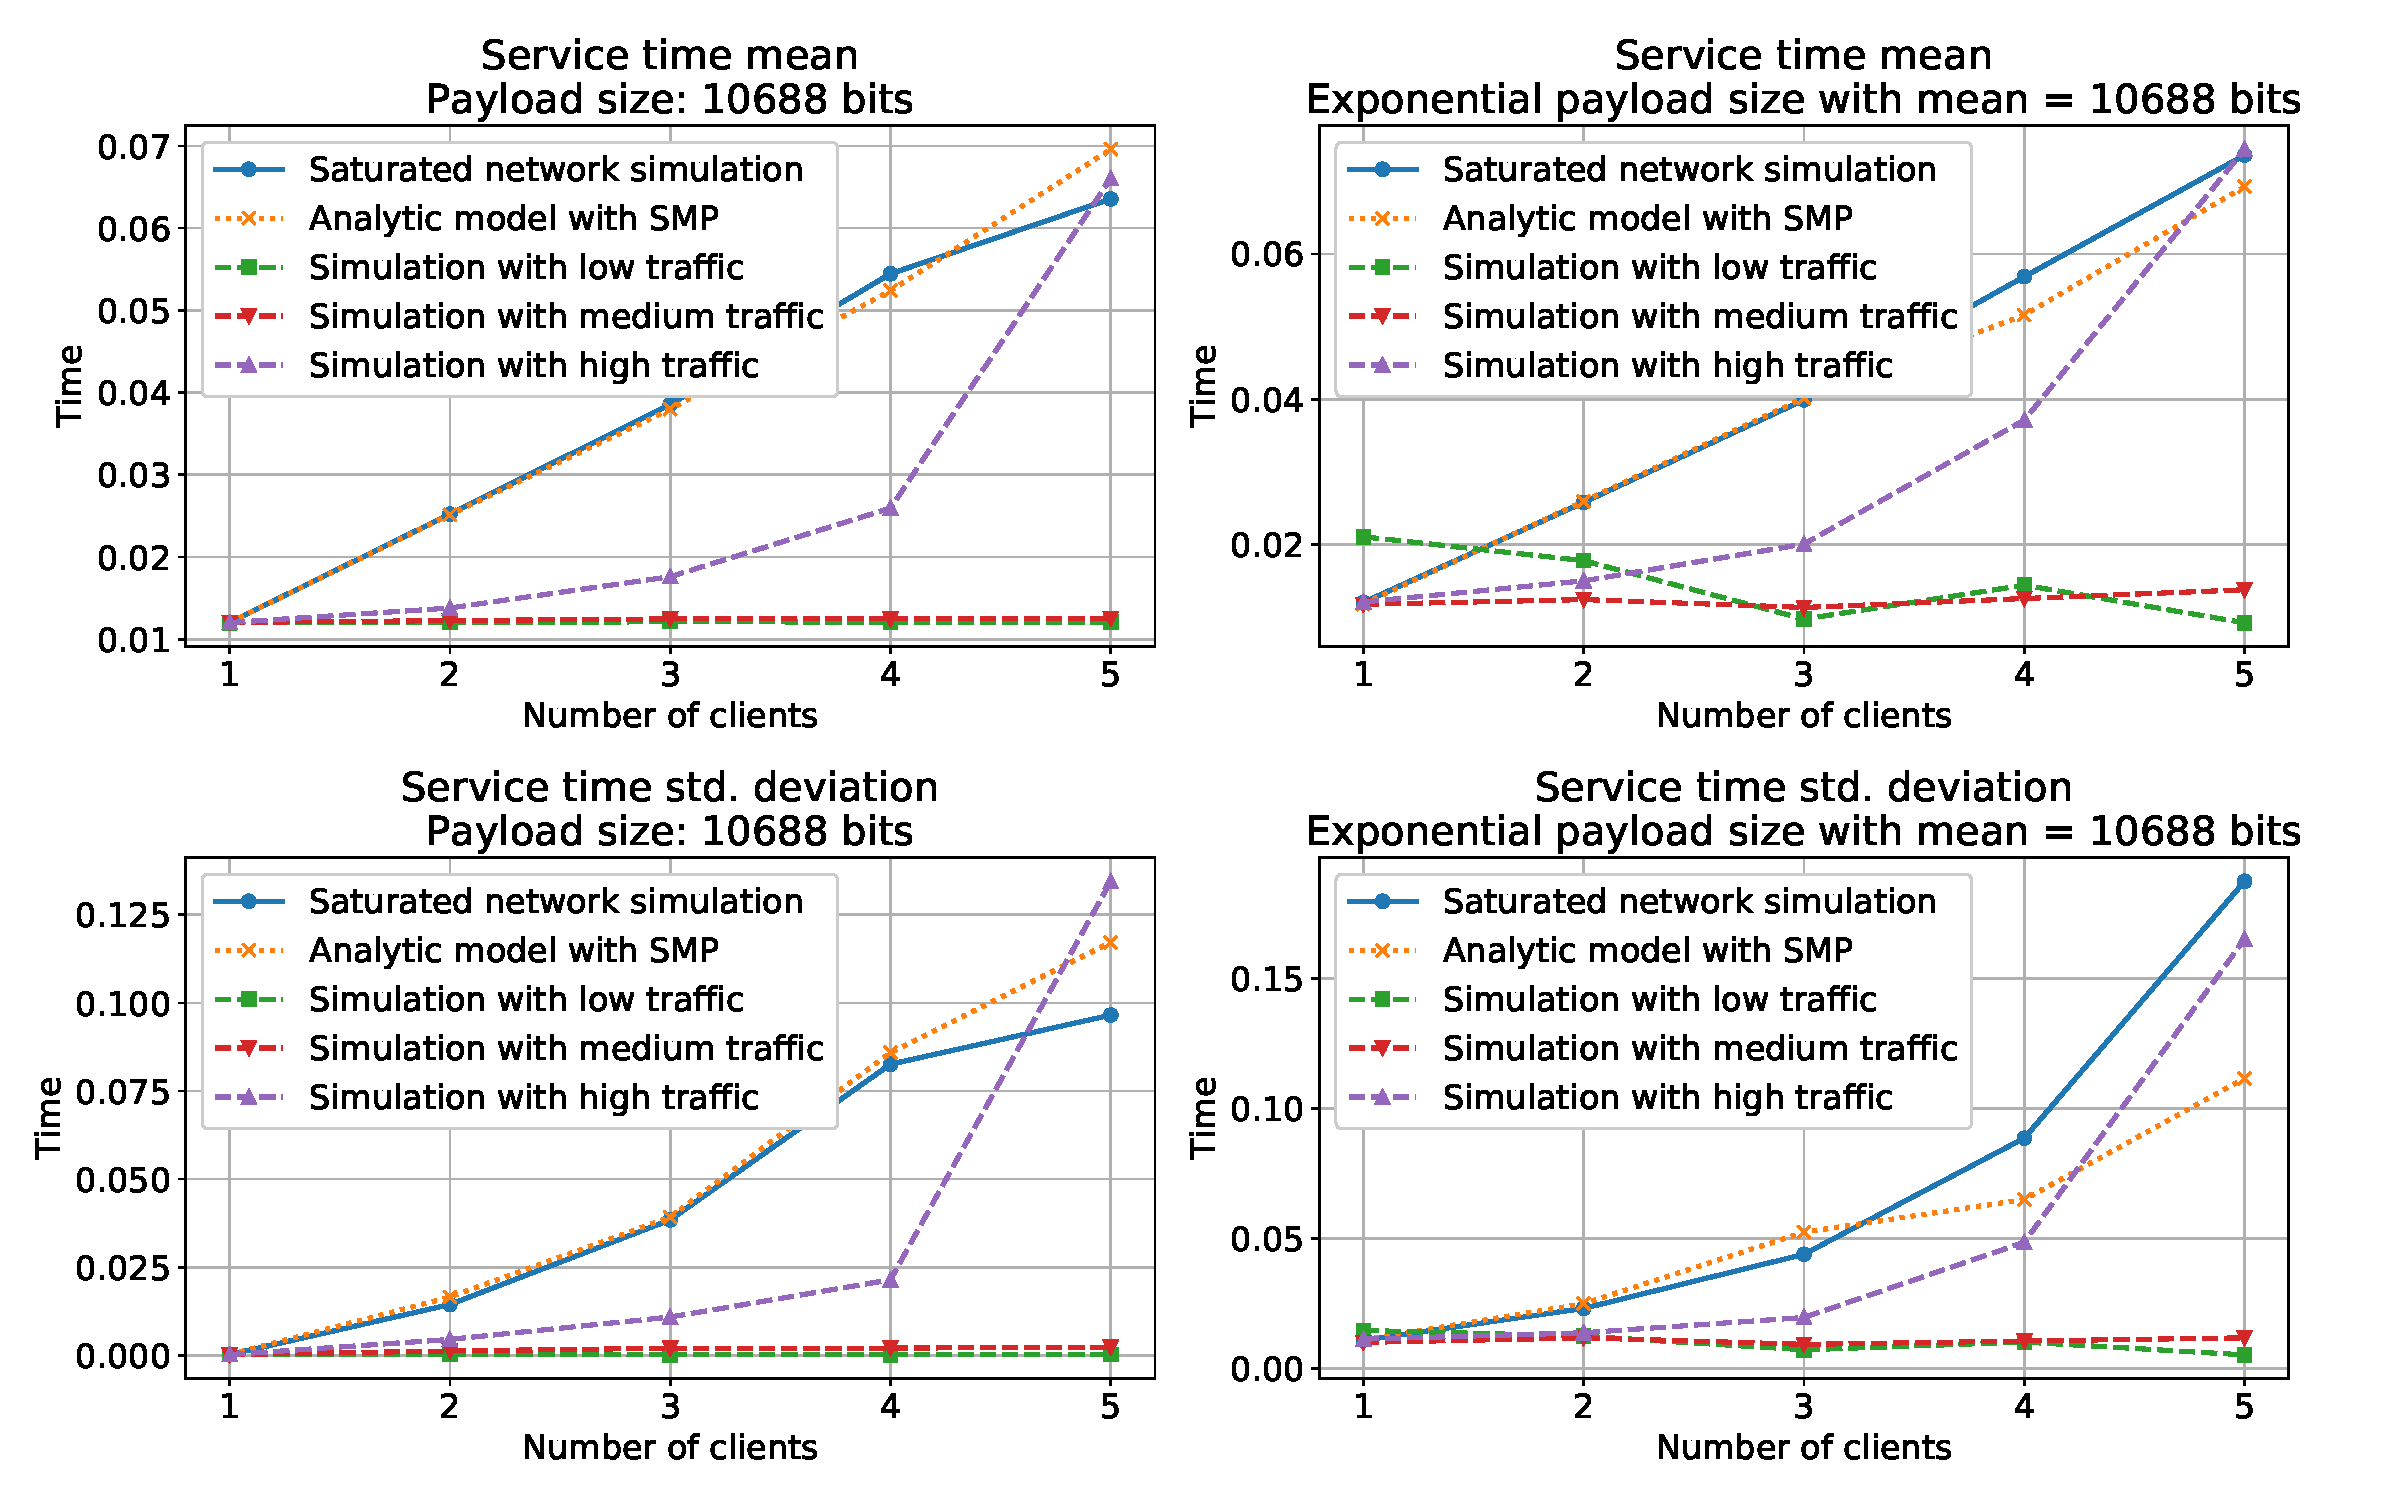
\includegraphics[scale=0.3]{chapter4/ch4_fitting_dcf_means.pdf}
  }
  \caption{Оценки средних значений и стандартных отклонений для беспроводных каналов IEEE 802.11}\label{fig:fitting_dcf_means}
\end{figure}

В \S~4 главы 4 приведены результаты численных экспериментов для моделирования сетей с каналами IEEE 802.11 и радиорелейными линиями. Для каналов IEEE 802.11 приведены результаты вычисления средних значений и стандартных отклонений для распределения задержек в беспроводных каналах, полученных с помощью имитационного моделирования сети и с помощью полумарковского случайного процесса (см. рис.~\ref{fig:fitting_dcf_means}). Показано, что для насыщенного режима полумарковский процесс дает хорошее приближение. В случае ненасыщенного режима среднее время передачи и его отклонение оказывается существенно ниже.

\begin{figure}[ht!]
  \centerfloat{
    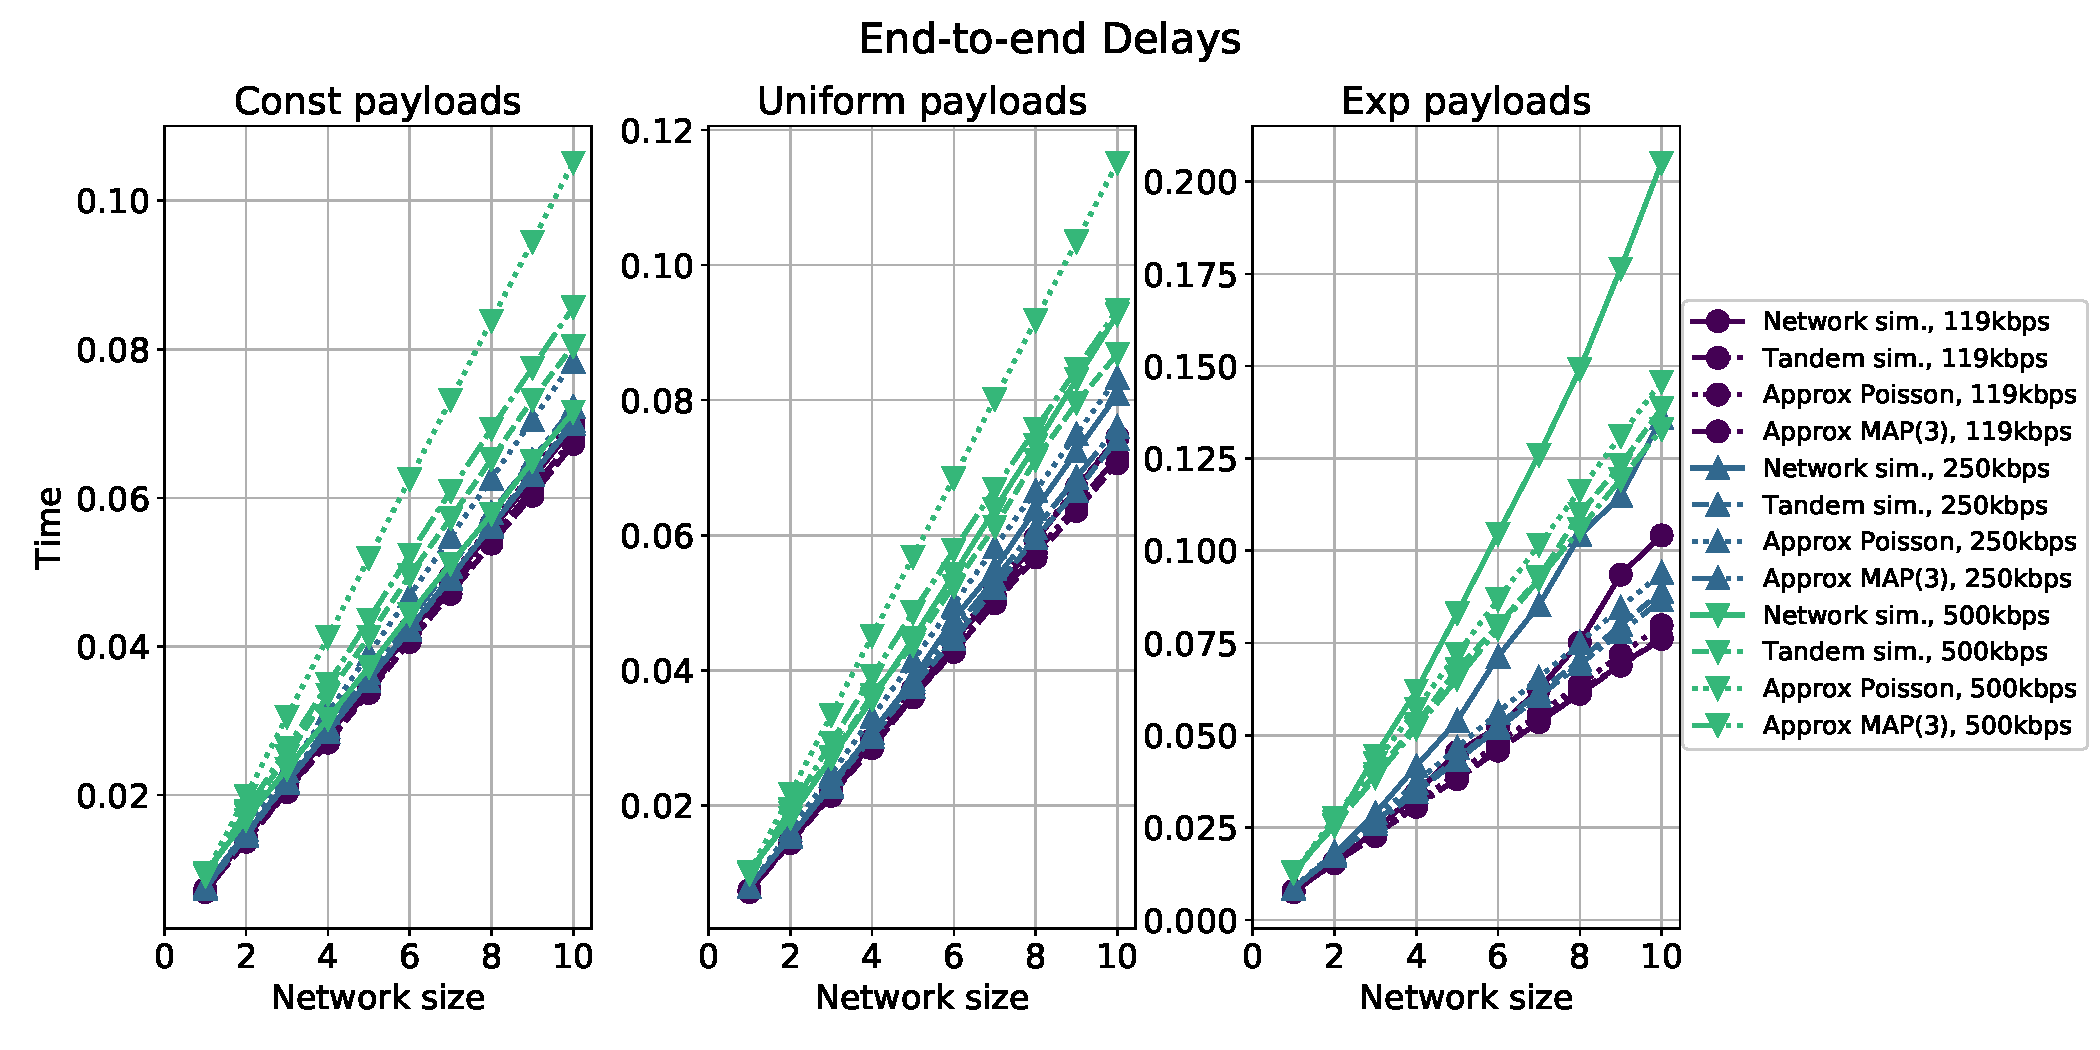
\includegraphics[scale=0.33]{chapter4/ch4_relay_delays.pdf}
  }
  \caption{Межконцевые задержки в сети с радиорелейными каналами}\label{fig:relay_means}
\end{figure}

\begin{figure}[ht!]
  \centerfloat{
    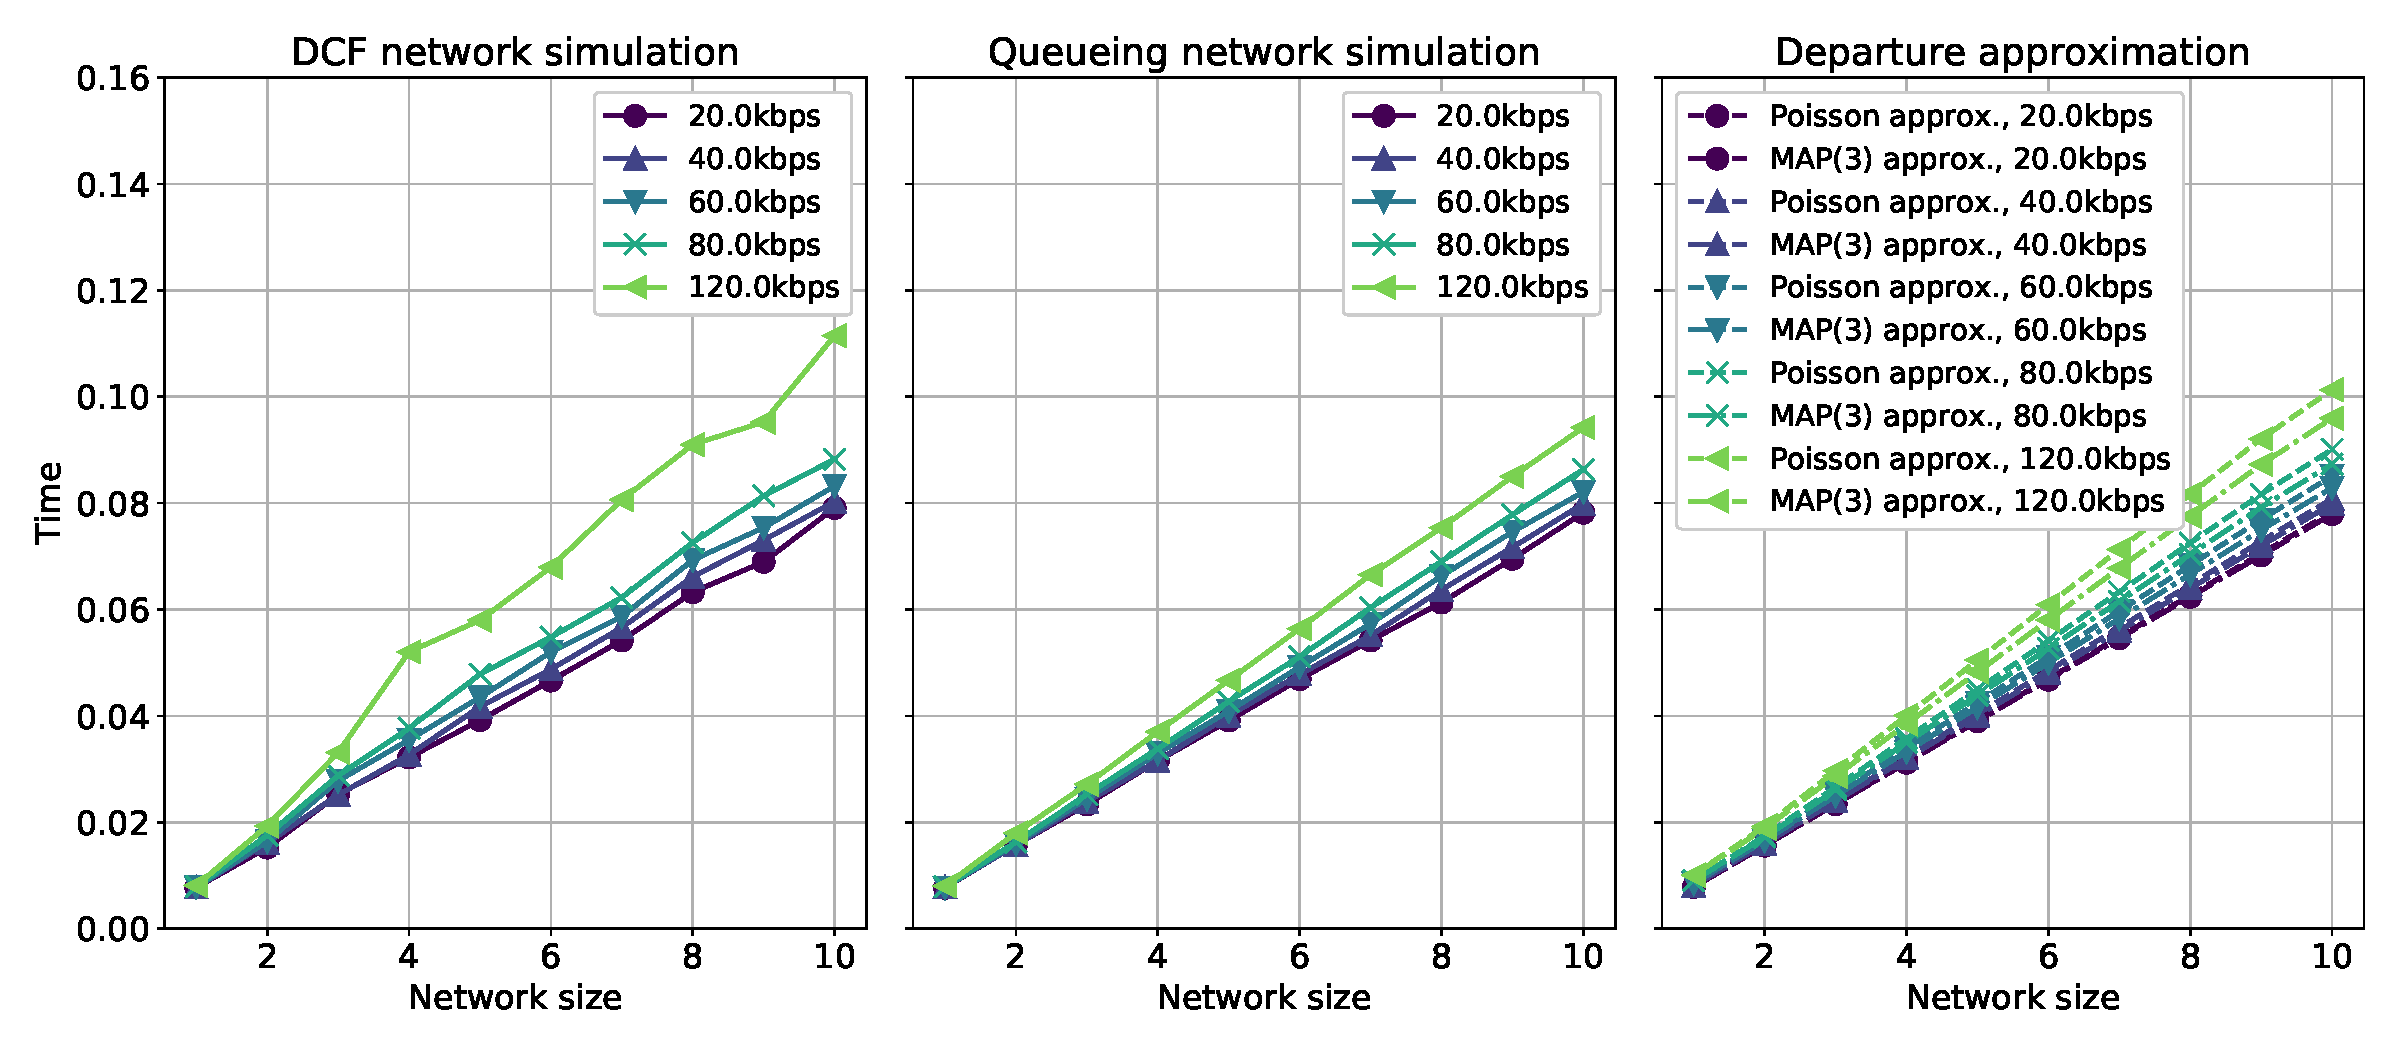
\includegraphics[scale=0.3]{chapter4/ch4_dcf_delays_noct_1.pdf}
  }
  \caption{Межконцевые задержки в сети с каналами IEEE 802.11}\label{fig:dcf_means}
\end{figure}

Межконцевые задержки в сети, длины очередей и прочие характеристики получены тремя способами: с помощью имитационной модели беспроводной сети, с помощью метода Монте-Карло для сети массового обслуживания с узлами MAP/PH/1/N и с помощью итерационного алгоритма с понижением размерности выходящих потоков. При аппроксимации выходящих потоков использовались MAP-потоки третьего и первого порядков (MAP первого порядка "--- это Пуассоновский простейший поток). Показано, что низкой и средней нагрузке при различных входящих потоках результаты всех трех методов оказываются очень близки, а при высокой нагрузке модель сети массового обслуживания дает несколько меньшие значения межконцевых задержек. Отмечается также, что для сети с радиорелейными каналами (см. рис.~\ref{fig:relay_means}) хороший результат дает приближение выходящих потоков MAP-потоком третьего порядка, а для сети с каналами CSMA/CA достаточно приближения выходящего потока простейшим пуассоновским потоком (см. рис.~\ref{fig:dcf_means}). Это являение объясняется тем, что передача одного и того же пакета разными узлами должно иметь одинаковую длительность для радиорелейной линии, но для каналов CSMA/CA, подверженных коллизиям, может отличаться.

В \S~5 главы 4 представлены результаты анализа производительности многошаговой сети с узлами IEEE 802.11g, полученные с помощью имитационного моделирования в системе OMNeT++ с пакетом INET, а также с помощью стенда из трех беспроводных маршрутизаторов MikroTik и Ubiquiti. В качестве источника трафика использовалась программа, моделирующая поток данных о прочитанных метках. Было экспериментально показано, что такая сеть может успешно справиться с передачей данных даже от тысячи считывателей.





В главе 5 представлены результаты проведенных в городе Казань экспериментов по внедрению системы радиочастотной идентификации в 2014 и 2020 годах. В \S~1 главы 5 приведена архитектура программного обеспечения разработанного RFID-считывателя и распределенной системы управления, кратко описаны основные программные компоненты и протоколы взаимодействия между ними. В \S~2 главы 5 даны краткие сведения об особенностях реализации системы управления на языках C/C++. В \S~3 приведено описание эксперимента 2014 года, в ходе которого разработанными RFID-считывателями было оборудовано две точки идентификации, а в центре обработки данных ГИБДД был размещен сервер, в котором собирались данные о прочитанных метках. Сами метки были установлены в автомобильные номера и ими были осноащены 920 автобусов. Эксперимент продолжался три зимних месяца, с декабря по февраль, в результате была получена вероятность успешной идентификации 92~\% и 95~\%. В ходе эксперимента были выявлены проблемы с перегруженной видеонаблюдением сетью, которые были решены добавлением кэширования на считывателях, но свидетельствуют о целесообразности построения недорогих выделенных беспроводных сетей для подключения считывателей. В \S~4 главы 5 описаны результаты протокольных испытаний, проведенный на полигоне в городе Казань. В ходе этих испытаний изучалась эффективность радиочастотной идентификации при проезде автомобилей на скоростях до 150~км/ч, а также при различных маневрах "--- следовании, обгоне. RFID-метки, разработанные ПАО <<Микрон>>, также были установлены в автомобильные номера. Во всех экспериментах все автомобили были успешно идентифицированы.

\FloatBarrier
\pdfbookmark{Заключение}{conclusion}                                  % Закладка pdf
В \underline{\textbf{заключении}} приведены основные результаты работы, которые заключаются в следующем:
%% Согласно ГОСТ Р 7.0.11-2011:
%% 5.3.3 В заключении диссертации излагают итоги выполненного исследования, рекомендации, перспективы дальнейшей разработки темы.
%% 9.2.3 В заключении автореферата диссертации излагают итоги данного исследования, рекомендации и перспективы дальнейшей разработки темы.
\begin{enumerate}
  \item Описан способ построения распределенной системы радиочастотной идентификации автомобилей, выделены факторы, влияющие на производительность системы;
  \item Представлены результаты численного исследования аналитической модели протокола EPC Gen2, показывающие целесообразность периодической смены считывателем опрашиваемого значения флага сессии и периодического сброса питания;
  \item Предложена имитационная модель системы радиочастотной идентификации автомобилей, учитывающая особенности распространения сигнала вблизи дороги, эффект Допплера, параметры антенных систем, настройки протокола EPC Gen.2;
  \item С помощью имитационного моделирования получены численные оценки вероятности идентификации быстро движущихся автомобилей при различных настройках протокола. Полученные результаты близко соотносятся с данными, полученными в ходе экспериментального внедрения системы, и показывают, что при определенных настройках можно добиться высокой вероятности идентификации быстро движущихся автомобилей с размещенными в номерных знаках метках;
  \item Описан способ построения распределений фазового типа для моделирования беспроводных каналов связи с использованием существующих стохастических моделей каналов;
  \item Предложена открытая сеть массового обслуживания с марковскими входными потоками, обслуживанием фазового типа и ограниченной памятью, повторными передачами и потерями пакетов из-за ошибок в канале, позволяющая моделировать беспроводную опорную сеть;
  \item Для беспроводных сетей с линейной топологией предложен метод оценки производительности с использованием систем массового обслуживания MAP/PH/1/n;
  \item Рассмотрен способ расчёта параметров производительности тандемных сетей массового обслуживания с узлами вида MAP/PH/1/n, позволяющий ограничить размерность модели за счет использования методов аппроксимации MAP-потоков обслуженных пакетов;
  \item Представлены численные результаты, показывающие адекватную точность предложенных методов моделирования беспроводных каналов связи и опорных беспроводных сетей с линейной топологией;
  \item Предложена архитектура промежуточного программного обеспечения для подключения большого количества географически разделенных RFID-считывателей к центру управления, обеспечивающего получение данных от считывателей, мониторинг и управление системой;
  \item Представлены результаты экспериментов по исследованию и внедрению системы радиочастотной иденификации автобусов в городе Казань 2014 и 2020 годов. Показано, что эффективность системы достигает 95~\%.
\end{enumerate}


\pdfbookmark{Литература}{bibliography}                                % Закладка pdf
% При использовании пакета \verb!biblatex! список публикаций автора по теме
% диссертации формируется в разделе <<\publications>>\ файла
% \verb!common/characteristic.tex!  при помощи команды \verb!\nocite!

\ifdefmacro{\microtypesetup}{\microtypesetup{protrusion=false}}{} % не рекомендуется применять пакет микротипографики к автоматически генерируемому списку литературы
\urlstyle{rm}                               % ссылки URL обычным шрифтом
\ifnumequal{\value{bibliosel}}{0}{% Встроенная реализация с загрузкой файла через движок bibtex8
  \renewcommand{\bibname}{\large \bibtitleauthor}
  \nocite{*}
  \insertbiblioauthor           % Подключаем Bib-базы
  %\insertbiblioexternal   % !!! bibtex не умеет работать с несколькими библиографиями !!!
}{% Реализация пакетом biblatex через движок biber
  % Цитирования.
  %  * Порядок перечисления определяет порядок в библиографии (только внутри подраздела, если `\insertbiblioauthorgrouped`).
  %  * Если не соблюдать порядок "как для \printbibliography", нумерация в `\insertbiblioauthor` будет кривой.
  %  * Если цитировать каждый источник отдельной командой --- найти некоторые ошибки будет проще.
  %
  %% authorvak
  \nocite{WINET_TCOMM2015}
  \nocite{QS_JPU2013}
  \nocite{QS_JITCS2013}
  \nocite{QS_TCOMM2012}

  %% authorwos - journals
  \nocite{RFID_JRFID2017}
  \nocite{WINET_IJPAM2016}
    
  % \nocite{vakbib1}%
  % \nocite{vakbib2}%
  %
  %% authorwos
  % \nocite{wosbib1}%
  \nocite{QS_ICAAPSP2020}
  \nocite{QS_ITMM2019}
  \nocite{RFID_IEEERFID2018}
  \nocite{RFID_SYNCHROINFO2018}
  \nocite{RFID_IEEERFID2017}
  \nocite{QS_AICT2017}
  \nocite{QS_ITMM2017}
  \nocite{QS_ITMM2016}
  \nocite{QS_DCCN2016_CCIS}
  \nocite{RFID_DCCN2016_CCIS}
  \nocite{RFIDCTRL_NETS2CARS2014}
  \nocite{RFIDTA2012}

  %
  %% authorscopus
  % \nocite{scbib1}%
  %
  %% authorpathent
  % \nocite{patbib1}%
  %
  %% authorprogram
  % \nocite{progbib1}%
  %
  %% authorconf
  % \nocite{confbib1}%
  % \nocite{confbib2}%
  %
  %% authorother
  % \nocite{bib1}%
  % \nocite{bib2}%

  \ifnumgreater{\value{usefootcite}}{0}{
    \begin{refcontext}[labelprefix={}]
      \ifnum \value{bibgrouped}>0
        \insertbiblioauthorgrouped    % Вывод всех работ автора, сгруппированных по источникам
      \else
        \insertbiblioauthor      % Вывод всех работ автора
      \fi
    \end{refcontext}
  }{
  \ifnum \totvalue{citeexternal}>0
    \begin{refcontext}[labelprefix=A]
      \ifnum \value{bibgrouped}>0
        \insertbiblioauthorgrouped    % Вывод всех работ автора, сгруппированных по источникам
      \else
        \insertbiblioauthor      % Вывод всех работ автора
      \fi
    \end{refcontext}
  \else
    \ifnum \value{bibgrouped}>0
      \insertbiblioauthorgrouped    % Вывод всех работ автора, сгруппированных по источникам
    \else
      \insertbiblioauthor      % Вывод всех работ автора
    \fi
  \fi
  %  \insertbiblioauthorimportant  % Вывод наиболее значимых работ автора (определяется в файле characteristic во второй section)
  \begin{refcontext}[labelprefix={}]
      \insertbiblioexternal            % Вывод списка литературы, на которую ссылались в тексте автореферата
  \end{refcontext}
  % Невидимый библиографический список для подсчёта количества внешних публикаций
  % Используется, чтобы убрать приставку "А" у работ автора, если в автореферате нет
  % цитирований внешних источников.
  \printbibliography[heading=nobibheading, section=0, env=countexternal, keyword=biblioexternal, resetnumbers=true]%
  }
}
\ifdefmacro{\microtypesetup}{\microtypesetup{protrusion=true}}{}
\urlstyle{tt}                               % возвращаем установки шрифта ссылок URL
